\chapter{\textsc{GPIO (General Purpose Input Output)}}

Le GPIO (General Purpose Input/Output) est une broche d'entrée ou sortie à usage générique. Les GPIOs sont groupées en ports de 8bits ou 16bits. Au sein d'un port ont peut accéder à chaque broche indépendamment en utilisant un masque (voir §2.2).

Les GPIOs sont configurés é l'aide de registres qui ont la dimension d'un port (8 ou 16 bits). Un port est donc juste un groupe de GPIOs qui permet une écriture simplifiée du code.


\section{Matériel}

Les GPIOs sont présents sur tous les microcontrôleurs en nombre plus ou moins grand selon le nombre de broches disponibles sur le boîtier. On choisit souvent un microcontrôleur en fonction du nombre de GPIO disponibles.

Le fonctionnement matériel du GPIO est décrit à la fig. \ref{fig:gpio}. 

\begin{figure}[htb]
  \centering
  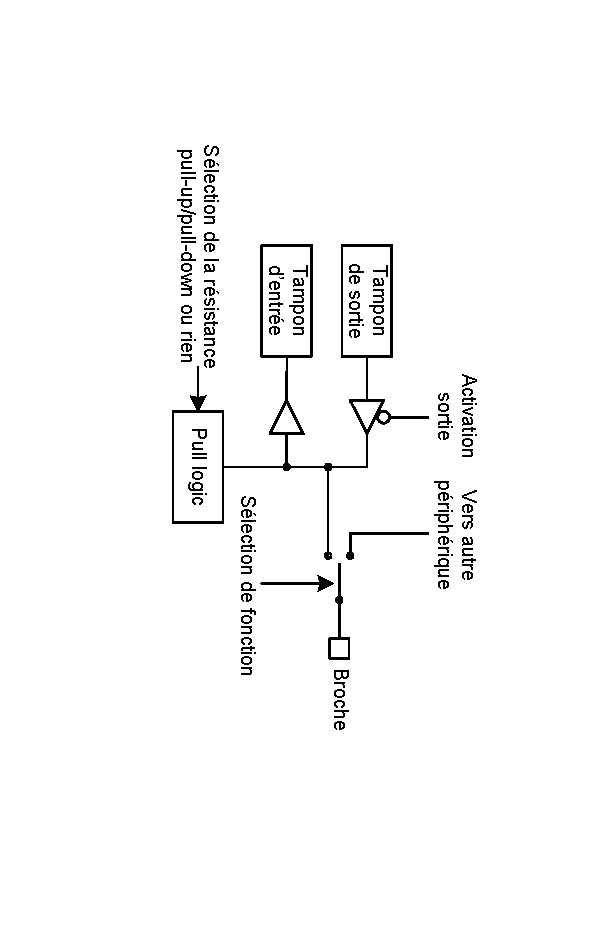
\includegraphics[angle=90, trim = 25mm 0mm 15mm 0mm, clip, width=14cm]{./Figures/gpio/Port.pdf}
  \rule{35em}{0.5pt}
  \caption[port GPIO]{Description matériel d'un GPIO}
  \label{fig:gpio}
\end{figure}

Il contient trois parties principales:
\begin{itemize}[label=\textbullet,font=\small]
\item Le circuit de sortie
\item Le circuit d'entrée
\item Un ou plusieurs commutateurs pour connecter la broche
\end{itemize}

Au delà du circuit de base décrit auparavant, il existe d'autres fonctions optionnelles dans les GPIO comme:
\begin{itemize}[label=\textbullet,font=\small]
\item synchronisation avec un signal ou une horloge 
\item circuit pour traiter des interruptions (voir ch. 4)
\item convertisseur de niveaux comme par exemple 3.3V - 5V
\item configuration de la puissance de l'amplificateur de sortie
\end{itemize}

\subsection{Input}

Dans la partie "entrée" du GPIO on trouve un tampon qui mémorise la valeur logique présente à l'entrée ainsi qu'un bloc pour sélectionner une résistance de pull-up ou pull-down. Ce bloc est très important car il est nécessaire pour éviter qu'une entrée se retrouve flottante. Si une entrée est laissée non-connectée (flottante) elle peut alors prendre n'importe quelle valeur et même changer de valeur aléatoirement au cours du temps. Pour éviter ce phénomène on doit utiliser une résistance placée selon le schéma suivant fig. \ref{fig:pullres}.

\begin{figure}[htb]
  \centering
  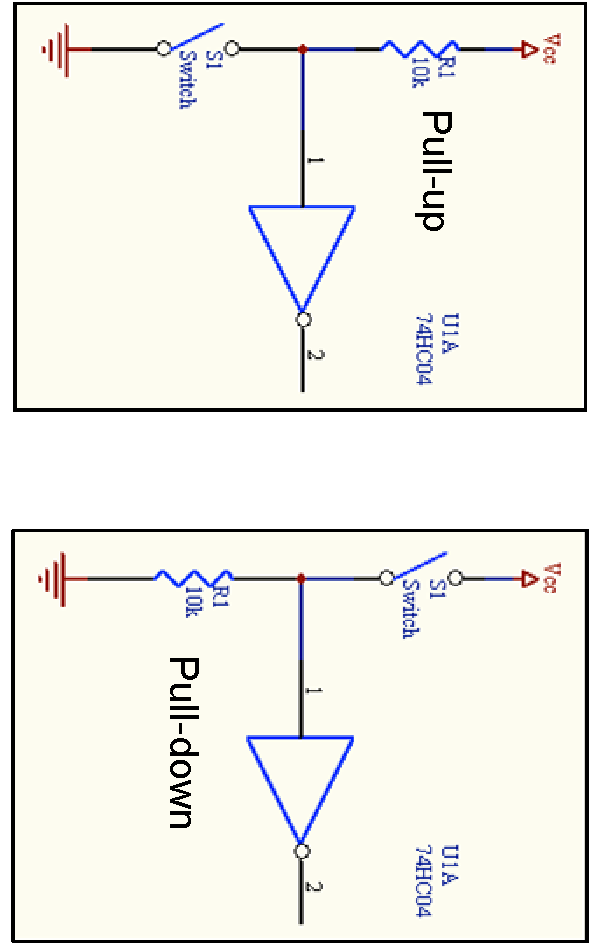
\includegraphics[angle=90, width=10cm]{./Figures/gpio/pullres.pdf}
  \rule{35em}{0.5pt}
  \caption[res pull]{Résistances de pull-up et pull-down}
  \label{fig:pullres}
\end{figure}

La valeur de cette résistance est choisie de manière optimale entre deux facteurs: i) le courant consommé VCC-GND qui doit être le plus faible possible quand l'interrupteur est fermé et ii) La vitesse à laquelle la résistance décharge la capacité d'entrée du circuit intégré CMOS lorsque l'interrupteur est ouvert. Les valeurs typiques se situent entre $10k\Omega$ et $100k\Omega$. Mais attention sous 3.3V, ça consommera lorsque l'interrupteur est fermé, entre $330\mu A$ et $33\mu A$ ce qui n'est pas négligeable!

Dans le cas particulier du MSP430F5529 la valeur typique des résistances de pull est de $35k\Omega$ ce qui provoque un courant de $86\mu A$ sous 3V. Il est donc avantageux de choisir un interrupteur poussoir plutôt que commutant pour minimiser le temps total de consommation. On peut aussi réduire la tension d'alimentation à 1.8V pour réduire le courant mais attention à la réduction de vitesse du microcontrôleur.

\subsection{Output}

Dans la partie "sortie" du GPIO on trouve un tampon qui mémorise la valeur logique que l'on veut sortir sur la broche ainsi qu'un amplificateur pour permettre au circuit de commuter la charge de sortie rapidement. Cette charge est souvent de type capacitive avec une valeur comprise entre 2pF et 10pF typiquement. On peut donc calculer le courant nécessaire pour charger cette capacité à 90\% dans un temps voulu. Ensuite on peut ajuster le courant, si disponible dans le GPIO, pour atteindre la vitesse recherchée.

\section{Logiciel}

Pour programmer les GPIOs on utilise des registres organisés en ports. Par exemple, dans la nomenclature Texas Instrument [réf], le port1 contient huit GPIO et on les nomme P1.0 à P1.7. On peut aussi utiliser le groupement par seize où la notation devient PA, PB, etc. PA est équivalent aux ports P0 et P1 regroupés alors que PB est équivalent aux ports P2 et P3. 

\subsection{Programmation par masque}

Comme les GPIO sont groupés en paquets de 8 ou 16 du point de vue logiciel, il faut un moyen pour programmer chaque GPIO individuellement. Cela signifie que si on modifie un GPIO, il ne faut surtout pas affecter les autres du même groupe. Un moyen d'arriver à ceci est d'utiliser un masque qui représente le bit désiré. Par exemple si on désire sélectionner le bit 3 on utilisera le masque BIT3 = 00001000 sur 8 bits (La numérotation commence é zéro). Si on désire sélectionner le bit 3 sur 16 bits alors le masque sera BIT3 = 0000000000001000.

Soit un registre (REG) de 8 bits servant à configurer 8 broches d'un microcontrôleur (fig \ref{fig:pxout}). 

\begin{figure}[htb]
  \centering
  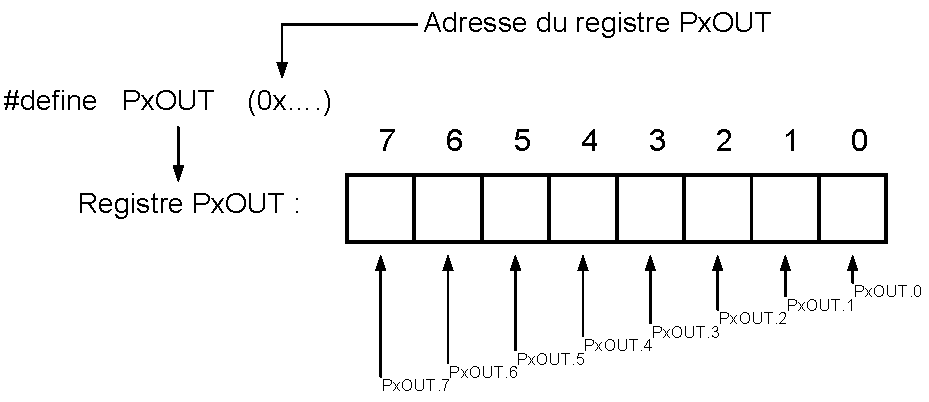
\includegraphics[angle=0, width=10cm]{./Figures/gpio/PxOUT.pdf}
  \rule{35em}{0.5pt}
  \caption[buff out]{Tampon de sortie}
  \label{fig:pxout}
\end{figure}

Pour mettre à 1 le bit 0 sans changer les bits 1 à 7 on peut utiliser la fonction OU; REG = REG OU BIT0 avec BIT0 = 00000001:

\lstset{style=customc}
\begin{lstlisting}
REG = REG | BIT0  //en C avec BIT0 = 0x01
REG |= BIT0		  //en C simplifié
\end{lstlisting}

On appelle cette technique le masquage. Pour mettre un bit à 0, il faut utiliser une autre fonction logique car le OU logique ne fait rien avec un zéro. Il est intéressant de résoudre ce problème par soi-même pour trouver la solution. On cherche donc à mettre un bit à 0 sans changer l'état logique des autres bits du port. Pour trouver la solution on peut partir d'un exemple et procéder par élimination:

\lstset{style=customc}
\begin{lstlisting}
REG = 0b00000011    //on désire mettre le premier bit à zéro sans influencer les autres
\\test avec OU:
REG = REG | BIT0  //ne fait rien donc ce n'est pas la solution
\\test avec ET:
REG = REG & BITO  //REG = 0b00000001 FAUX ça ne marche pas non plus
\end{lstlisting}

Mais si on avait inversé BIT0 alors ça aurait marché:

\lstset{style=customc}
\begin{lstlisting}
REG = REG & ~BITO   //REG = 0b00000010 JUSTE 
REG &= ~BIT0         //en C simplifié
\end{lstlisting}

On constate donc qu'il faut utiliser la fonction duale mais avec une inversion préalable. Ceci convient pour l'écriture dans un registre mais qu'en est-il de la lecture? Comment pourrait-on lire un GPIO parmi tous les bits d'un port?

La réponse est similaire au test d'un bit dans un mot en langage C. Prenons comme exemple la lecture, ou test, du BIT0 dans REG et procédons par élimination. Il faut trouver la fonction désirée avec par exemple REG = 00000011 et BIT0 = 00000001:

\lstset{style=customc}
\begin{lstlisting}
//essai avec OU avec REG = 0b00000011 et BIT0 = 0b00000001:
TEST_BIT0 = REG | BIT0  //TEST_BIT0 = 0b00000011 FAUX
//et si REG = 0b00000010
TEST_BIT0 = REG | BIT0  //TEST_BIT0 = 0b00000011 FAUX

//Il est clair que ça ne marche pas avec OU essayons avec ET:
TEST_BIT0 = REG & BIT0  //TEST_BIT0 = 0b00000001 JUSTE
//et si REG = 0b00000010
TEST_BIT0 = REG & BIT0  //TEST_BIT0 = 0b00000000 JUSTE
\end{lstlisting}

Donc le test ou lecture d'une valeur s'effectue avec l'opérateur logique ET. Dans le cas d'un test en C, on doit se rappeler que le résultat est VRAI pour toute valeur de TEST\_BITx différente de zéro. Il est faux si et seulement si TEST\_BITx = 0. Ceci provient du fait que la variable C la plus petite est de 8 bits. Il n'y a pas de variable de 1 bit en C. 

\subsection{écriture dans un registre}

Soit le registre REG d'une longueur de 8 bits. Pour écrire la valeur logique 1 dans le registre on utilise la fonction OU entre le registre et le masque du bit voulu. Pour écrire un 0 logique on utilise la fonction ET entre le registre et le masque du bit voulu inversé, exemples:

\lstset{style=customc}
\begin{lstlisting}
//Mise à 1 du bit zéro:
REG = REG | BIT0    //en C avec BIT0 = 0x01
REG |= BIT0		    //en C simplifié

//Mise à 0 du bit zéro:
REG = REG & ~BITO   //REG = 0b00000010 JUSTE 
REG &= ~BIT0         //en C simplifié
\end{lstlisting}

Pour la mise à 1 ou 0 simultanée de plusieurs bits on utilise le OU pour sommer les masques et créer un masque contenant les deux bits. Exemple: BIT3 | BIT0 = 00001001:

\lstset{style=customc}
\begin{lstlisting}
//Mise à 1 du bit zéro et trois simultanément:
REG |= BIT0 | BIT3

//Mise à 0 du bit zéro et trois simultanément:
REG &= ~BIT0 | BIT3
\end{lstlisting}

\subsection{Lecture d'un registre}

Pour lire un registre on compare le registre avec le masque du bit voulu en utilisant la fonction ET: 

\lstset{style=customc}
\begin{lstlisting}
//Lecture du BIT3 uniquement:
TEST_REG = REG & BIT3; // BIT3 = 0b00001000
\end{lstlisting}

Le résultat de cette affectation sera donc 0 si le BIT3 est à zéro et 8 si le BIT3 est à 1. Pour lire plusieurs bits à la fois on peut, comme pour l'écriture, créer un masque combiné. Exemple, on veut lire le bit 5 et le bit 2 simultanément:

\lstset{style=customc}
\begin{lstlisting}
//Lecture du BIT5 et du BIT2:
TEST_REG = REG & (BIT5 | BIT2); // BIT5 | BIT2 = 0b00100100
\end{lstlisting}

\section{Configuration des GPIO}

Avant de pouvoir utiliser un GPIO il faut le configurer. Cela inclut principalement:

\begin{itemize}[label=\textbullet,font=\small]
\item Le multiplexeur d'entrée
\item La fonction entrée ou sortie
\item La résistance de pull-up ou pull-down lorsqu'on est en entrée
\end{itemize}

Pour les configurer on doit trouver leurs adresses physiques qui les identifient à l'intérieur du circuit intégré. Ces adresses peuvent être trouvées dans la documentation du microcontrôleur mais souvent elles sont fournies sous forme de constantes dans une librairie qu'on peut inclure dans le code C.

\lstset{style=customc}
\begin{lstlisting}
#include <msp430.h>

#define P1IN  (PAIN_L)       /* Port 1 Input */
#define P1OUT (PAOUT_L)      /* Port 1 Output */
#define P1DIR (PADIR_L)      /* Port 1 Direction */
#define P1REN (PAREN_L)      /* Port 1 Resistor Enable */
#define P1DS  (PADS_L)       /* Port 1 Drive Strength */
#define P1SEL (PASEL_L)      /* Port 1 Selection */
\end{lstlisting}

Exemple de configuration du port P1.2 et P1.5 en sortie:

\lstset{style=customc}
\begin{lstlisting}
P1SEL &= ~BIT5 & ~BIT2;  // Reset P1.2 et P1.5 to select GPIO
P1DIR |=  BIT5 | BIT2;   // Set P1.2 et P1.5 to output direction
//Option: ajouter le P1DS pour changer le courant de sortie

//Puis écriture sur les sorties P1.5 et P1.2 d'un 1 logique:
P1OUT |= BIT5 | BIT2;
\end{lstlisting}

Exemple de configuration du port P1.2 et P1.5 en entrée:

\lstset{style=customc}
\begin{lstlisting}
P1SEL &= ~(BIT5 | BIT2);  // Reset P1.2 et P1.5 to select GPIO
P1DIR &= ~(BIT5 | BIT2);  // Reset P1.2 et P1.5 to input direction
//Option: ajouter les résistances de pull
P1OUT |= BIT5 | BIT2;    // Sélection de la résistance
P1REN |= BIT5 | BIT2;    // Activation de la résistance

//Puis lecture de l'entrée P1.5 et P1.2:
TEST_REG = P1IN & (BIT5 | BIT2);
\end{lstlisting}

